\documentclass{report}
\setlength{\parskip}{\baselineskip}%
\usepackage{amsmath}
\usepackage{amsfonts,stmaryrd,amssymb} % Math packages

\usepackage{enumerate} % Custom item numbers for enumerations
\usepackage{fontawesome}
\usepackage{setspace}
\usepackage{hyperref}
\usepackage{enumitem}
\usepackage{multicol}
\usepackage{xhfill}
\usepackage[p,osf]{cochineal}
\usepackage[scale=.95,type1]{cabin}
\usepackage[cochineal,bigdelims,cmintegrals,vvarbb]{newtxmath}
\usepackage[zerostyle=c,scaled=.94]{newtxtt}
\usepackage[cal=boondoxo]{mathalfa}
\usepackage[export]{adjustbox}
\usepackage{vwcol}  
\usepackage{fancyhdr}
\DeclareSymbolFont{yhlargesymbols}{OMX}{yhex}{m}{n}
\DeclareMathAccent{\wideparen}{\mathord}{yhlargesymbols}{"F3}

\hypersetup{
	colorlinks=false,
	linkcolor=black,
	filecolor=black,      
	urlcolor=black,
	pdftitle={Overleaf Example},
	pdfpagemode=FullScreen,
	urlbordercolor=white,
}

\urlstyle{same}


	
\newenvironment{cequation}{
	\makeatletter
	\setbool{@fleqn}{false}
	\makeatother
	\begin{equation*}
		}{\end{equation*}}
		
\newcommand{\sol}{\noindent\textbf{Solution:} }
%----------------------------------------------------------------------------------------

\newcommand{\exercise}[1]{%
	\subsection*{\faPencil\ \ Exercise #1\hspace{0.5em}\xrfill[0.175\baselineskip]{1pt}}
}

\newcommand{\practice}[1]{%
	\subsection*{\faFlag\ \ Practice #1\hspace{0.5em}\xrfill[0.175\baselineskip]{1pt}}
}

\newcommand{\revision}[1]{%
	\section*{\faGears\ \ Revision Exercise #1\hspace{0.5em}\xrfill[0.175\baselineskip]{1pt}}
}

\usepackage[ruled]{algorithm2e} % Algorithms

\usepackage[framemethod=tikz]{mdframed} % Allows defining custom boxed/framed environments

\usepackage{listings} % File listings, with syntax highlighting
\lstset{
	basicstyle=\ttfamily, % Typeset listings in monospace font
}

%----------------------------------------------------------------------------------------
%	DOCUMENT MARGINS
%----------------------------------------------------------------------------------------

\usepackage{geometry} % Required for adjusting page dimensions and margins

\geometry{
	paper=a4paper, % Paper size, change to letterpaper for US letter size
	top=2.5cm, % Top margin
	bottom=3cm, % Bottom margin
	left=2.5cm, % Left margin
	right=2.5cm, % Right margin
	headheight=14pt, % Header height
	footskip=1.5cm, % Space from the bottom margin to the baseline of the footer
	headsep=1.2cm, % Space from the top margin to the baseline of the header
	%showframe, % Uncomment to show how the type block is set on the page
}

%----------------------------------------------------------------------------------------
%	FONTS
%----------------------------------------------------------------------------------------

\usepackage[utf8]{inputenc} % Required for inputting international characters
\usepackage[T1]{fontenc} % Output font encoding for international characters

%----------------------------------------------------------------------------------------
%	COMMAND LINE ENVIRONMENT
%----------------------------------------------------------------------------------------

% Usage:
% \begin{commandline}
%	\begin{verbatim}
%		$ ls
%		
%		Applications	Desktop	...
%	\end{verbatim}
% \end{commandline}

\mdfdefinestyle{commandline}{
	leftmargin=10pt,
	rightmargin=10pt,
	innerleftmargin=15pt,
	middlelinecolor=black!50!white,
	middlelinewidth=2pt,
	frametitlerule=false,
	backgroundcolor=black!5!white,
	frametitle={Command Line},
	frametitlefont={\normalfont\sffamily\color{white}\hspace{-1em}},
	frametitlebackgroundcolor=black!50!white,
	nobreak,
}

% Define a custom environment for command-line snapshots
\newenvironment{commandline}{
	\medskip
	\begin{mdframed}[style=commandline]
		}{
	\end{mdframed}
	\medskip
}

%----------------------------------------------------------------------------------------
%	FILE CONTENTS ENVIRONMENT
%----------------------------------------------------------------------------------------

% Usage:
% \begin{file}[optional filename, defaults to "File"]
%	File contents, for example, with a listings environment
% \end{file}

\mdfdefinestyle{file}{
	innertopmargin=1.6\baselineskip,
	innerbottommargin=0.8\baselineskip,
	topline=false, bottomline=false,
	leftline=false, rightline=false,
	leftmargin=2cm,
	rightmargin=2cm,
	singleextra={%
		\draw[fill=black!10!white](P)++(0,-1.2em)rectangle(P-|O);
		\node[anchor=north west]
		at(P-|O){\ttfamily\mdfilename};
		%
		\def\l{3em}
		\draw(O-|P)++(-\l,0)--++(\l,\l)--(P)--(P-|O)--(O)--cycle;
		\draw(O-|P)++(-\l,0)--++(0,\l)--++(\l,0);
	},
	nobreak,
}

% Define a custom environment for file contents
\newenvironment{file}[1][File]{ % Set the default filename to "File"
	\medskip
	\newcommand{\mdfilename}{#1}
	\begin{mdframed}[style=file]
		}{
	\end{mdframed}
	\medskip
}

%----------------------------------------------------------------------------------------
%	NUMBERED QUESTIONS ENVIRONMENT
%----------------------------------------------------------------------------------------

% Usage:
% \begin{question}[optional title]
%	Question contents
% \end{question}

\mdfdefinestyle{question}{
	innertopmargin=1.2\baselineskip,
	innerbottommargin=0.8\baselineskip,
	roundcorner=5pt,
	nobreak,
	singleextra={%
		\draw(P-|O)node[xshift=1em,anchor=west,fill=white,draw,rounded corners=3pt]{%
			\faCaretRight\ \textbf{Example \theQuestion\questionTitle}};
	},
}

\newcounter{Question} % Stores the current question number that gets iterated with each new question

% Define a custom environment for numbered questions
\newenvironment{question}[1][\unskip]{
	\bigskip
	\stepcounter{Question}
	\newcommand{\questionTitle}{~#1}
	\begin{mdframed}[style=question]
		}{
	\end{mdframed}
	\medskip
}

%----------------------------------------------------------------------------------------
%	SOLUTIONS ENVIRONMENT
%----------------------------------------------------------------------------------------

% Usage:
% \begin{solution}
%	Solution contents
% \end{solution}

\mdfdefinestyle{solution}{
	innertopmargin=1.2\baselineskip,
	innerbottommargin=0.8\baselineskip,
	roundcorner=5pt,
	nobreak,
	singleextra={%
		\draw(P-|O)node[xshift=1em,anchor=west,fill=white,draw,rounded corners=5pt]{解};
	},
}

% Define a custom environment for solutions
\newenvironment{solution}{
	\begin{mdframed}[style=solution]
		}{
	\end{mdframed}
}

%----------------------------------------------------------------------------------------
%	WARNING TEXT ENVIRONMENT
%----------------------------------------------------------------------------------------

% Usage:
% \begin{warn}[optional title, defaults to "Warning:"]
%	Contents
% \end{warn}

\mdfdefinestyle{warning}{
	topline=false, bottomline=false,
	leftline=false, rightline=false,
	nobreak,
	singleextra={%
		\draw(P-|O)++(-0.5em,0)node(tmp1){};
		\draw(P-|O)++(0.5em,0)node(tmp2){};
		\fill[black,rotate around={45:(P-|O)}](tmp1)rectangle(tmp2);
		\node at(P-|O){\color{white}\scriptsize\bf !};
		\draw[very thick](P-|O)++(0,-1em)--(O);%--(O-|P);
	}
}

% Define a custom environment for warning text
\newenvironment{warn}[1][Warning:]{ % Set the default warning to "Warning:"
	\medskip
	\begin{mdframed}[style=warning]
		\noindent{\textbf{#1}}
		}{
	\end{mdframed}
	\vspace{-0.5cm}
}

%----------------------------------------------------------------------------------------
%	INFORMATION ENVIRONMENT
%----------------------------------------------------------------------------------------

% Usage:
% \begin{info}[optional title, defaults to "Info:"]
% 	contents
% 	\end{info}

\mdfdefinestyle{info}{%
	topline=false, bottomline=false,
	leftline=false, rightline=false,
	nobreak,
	singleextra={%
		\fill[black](P-|O)circle[radius=0.6em];
		\node at(P-|O){\color{white}\scriptsize\bf \faInfo};
		\draw[very thick](P-|O)++(0,-0.8em)--(O);%--(O-|P);
	}
}

% Define a custom environment for information
\newenvironment{info}[1][Info:]{ % Set the default title to "Info:"
	\medskip
	\begin{mdframed}[style=info]
		\noindent{\textbf{#1}}
		}{
	\end{mdframed}
	\vspace{-0.5cm}
	
}

\mdfdefinestyle{explore}{%
	topline=false, bottomline=false,
	leftline=false, rightline=false,
	nobreak,
	singleextra={%
		\fill[black](P-|O)circle[radius=0.6em];
		\node at(P-|O){\color{white}\scriptsize\bf \faFlask};
		\draw[very thick](P-|O)++(0,-0.8em)--(O);%--(O-|P);
	}
}

% Define a custom environment for warning text
\newenvironment{explore}[1][Exploration Activity:]{ % Set the default warning to "Warning:"
	\medskip
	\begin{mdframed}[style=explore]
		\noindent{\large\textbf{#1}}
		}{
	\end{mdframed}
	\vspace{-0.5cm}
}

\mdfdefinestyle{think}{%
	topline=false, bottomline=false,
	leftline=false, rightline=false,
	nobreak,
	singleextra={%
		\fill[black](P-|O)circle[radius=0.6em];
		\node at(P-|O){\color{white}\scriptsize\bf \faQuestion};
		\draw[very thick](P-|O)++(0,-0.8em)--(O);%--(O-|P);
	}
}

% Define a custom environment for warning text
\newenvironment{think}[1][Think about It:]{ % Set the default warning to "Warning:"
	\medskip
	\begin{mdframed}[style=think]
		\noindent{\large\textbf{#1}}
		}{
	\end{mdframed}
	\vspace{-0.5cm}
}



\usepackage{tabularx}
\newcolumntype{Y}{>{\centering\arraybackslash}X}

\begin{document}
\pagestyle{fancy}
%... then configure it.
\fancyhead{} % clear all header fields
\fancyhead[RO,LE]{\thepage}
\fancyhead[LO,RE]{\leftmark}
\fancyfoot{} % clear all footer fields

\fancyfoot[LO,RE]{Dong Zong Addmath Textbook Senior 1 Volume II}
\fancyfoot[RO,RE]{\thepage}

\onehalfspacing
\setcounter{chapter}{8}

\chapter{Trigonometric Functions of Arbitrary Angles}

\section{Trigonometric Functions of Arbitrary Angles}

In Chapter 8, we extended the concept of angle by defining angle using ray rotation. Putting the direction and amount of rotation into consideration, we know that there are positive angles, negative angles, and zero angles (0°) of any size, collectively referred to as arbitrary angles. Next, we will discuss angles in a Cartesian coordinate system.

\subsection*{Angles and Quadrants}

In a plane, any angle can be moved so that the vertex of the angle coincides with the origin of the Cartesian coordinate system, and the initial side of the angle lies on the positive x-axis. With that, the quadrant to which the terminal side of the angle belongs determines which quadrant the angle is in (or to which quadrant the angle belongs). If the terminal side of the angle lies on the coordinate axes, then the angle does not belong to any quadrant. For example:
\vspace{-1em}
\begin{enumerate}[label=(\arabic*)]
    \item As shown in figure (a), $30^\circ$ and $390^\circ$ are both angles in the first quadrant.
    \item As shown in figure (b), $120^\circ$ and $-240^\circ$ are both angles in the second quadrant.
    \item As shown in figure (c), $-1$ rad and $(-2\pi + 1)$ rad are both angles in the fourth quadrant.
    \item As shown in figure (d), $\dfrac{3\pi}{2}$ rad and $-90^\circ$ do not belong to any quadrant.
\end{enumerate}

\begin{center}
    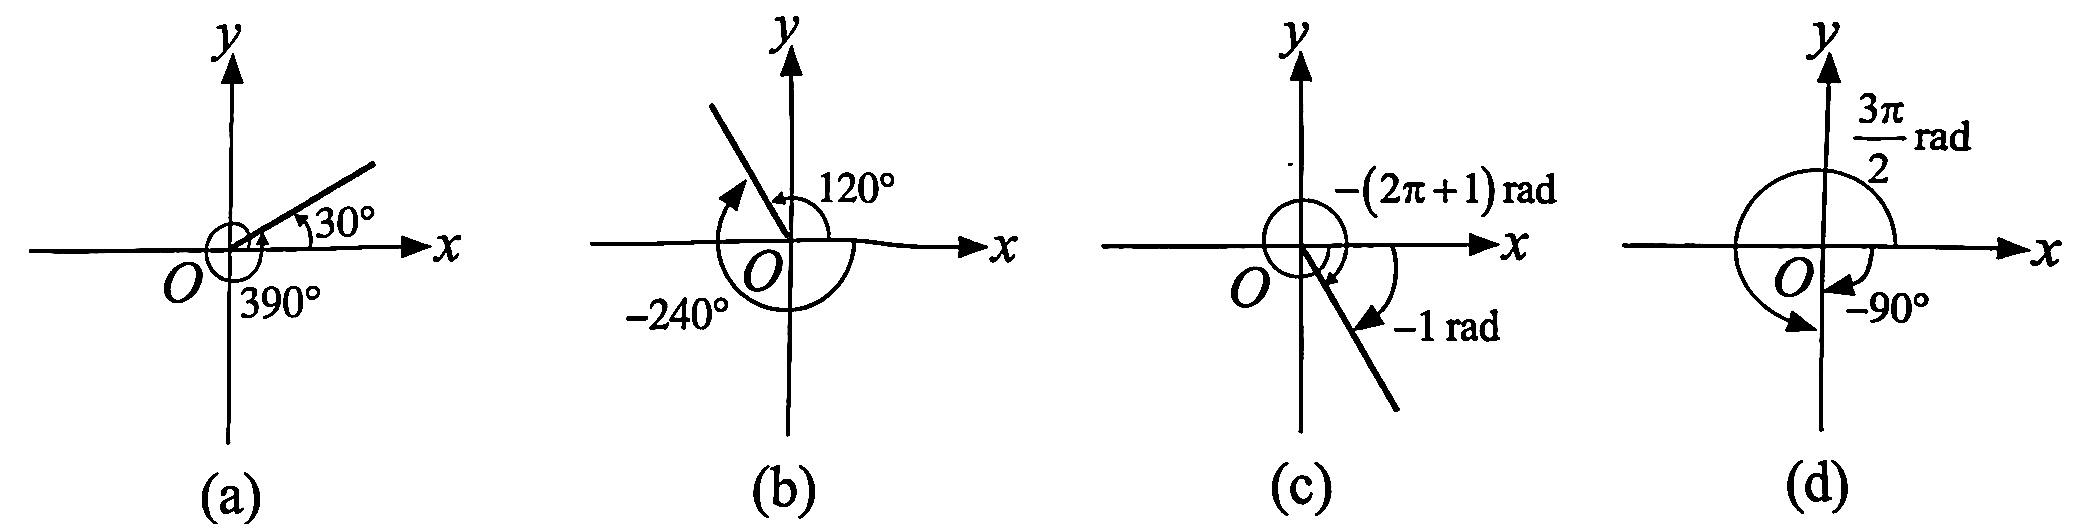
\includegraphics[width=0.8\textwidth]{assets/9-1.jpg}
\end{center}
\vspace{-1em}

\begin{think}
    Are "acute angle", "angle in the first quadrant", and "angle that is less than $90^\circ$" the same thing?
\end{think}

In this chapter, if not specified, the angles that we will discuss are angles of which the vertex is at the origin, and the initial side lies on the positive x-axis.

In the four sets of angles shown in the figures above, their initial and terminal sides are all the same. In fact, any angle $\theta$ that rotates one full round clockwise or counterclockwise will coincide with original terminal side, i.e. the terminal side of $\theta = 360^\circ$ or $\theta + (-360^\circ)$ will have the same terminal side as $\theta$. Using the same logic, we can conclude that: the angle $k \cdot 360^\circ + \circ$ will have the same terminal side as $\theta$ for $k \in \mathbb{Z}$.

\begin{question}
    Determine the quadrant to which the angle belongs.
    \vspace{-1em}
    \begin{multicols}{2}
        \begin{enumerate}[label=(\alph*)]
            \item $1020^\circ$
            \item $\dfrac{9}{4}\pi$
        \end{enumerate}
    \end{multicols}

    \sol{}
    \begin{multicols}{2}
        \begin{enumerate}[label=(\alph*)]
            \item $1020^\circ = 2(360^\circ) + 300^\circ$
                
            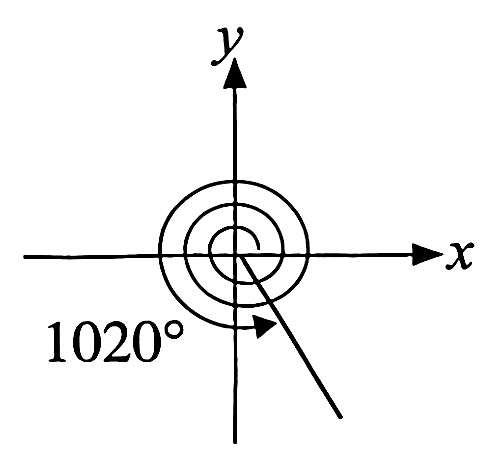
\includegraphics[width=0.2\textwidth]{assets/9-2.jpg}
            
            $\therefore 1020^\circ$ belongs to the fourth quadrant.
            \columnbreak

            \item $\dfrac{9}{4}\pi = 2\pi + \dfrac{\pi}{4}$
                
            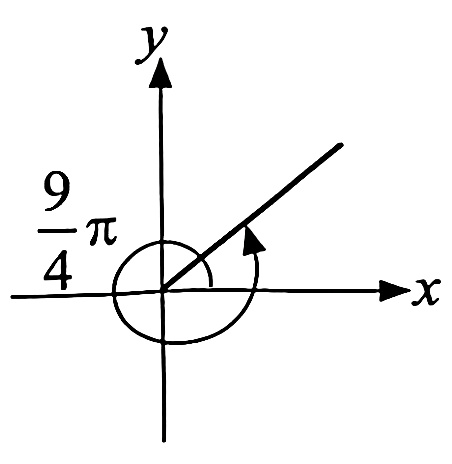
\includegraphics[width=0.2\textwidth]{assets/9-3.jpg}
            
            $\therefore \dfrac{9}{4}\pi$ belongs to the first quadrant.
        \end{enumerate}
    \end{multicols}
\end{question}

\practice{9.1a}
\begin{enumerate}
    \item Determine the quadrant to which the angle belongs.
    \begin{multicols}{4}
        \begin{enumerate}[label=(\alph*)]
            \item $\dfrac{2\pi}{3}$
            \item $740^\circ 50'$
            \item $-\dfrac{4\pi}{9}$
            \item $-135^\circ$
        \end{enumerate}
    \end{multicols}
    \item If $360^\circ < \theta < 450^\circ$, which quadrant does $\theta$ belong to?
    \item Given that $0^\circ < \theta < 360^\circ$ (i.e. $0 < \theta < 2\pi$), Find the angle $\theta$ with the same terminal side as the following angles:
    \begin{multicols}{4}
        \item $560^\circ 24'$
        \item $-15^\circ$
        \item $-1000^\circ$
        \item $\dfrac{12}{5}\pi$
    \end{multicols}
\end{enumerate}

\subsection*{Definition of Trigonometry Functions of Arbitrary Angles}

We have learned the trigonometric functions of acute angles: In a right triangle, the acute angle is the independent variable while the ratio of the sides is the value of the function.

Actually, now that we are discussing angles in a Cartesian coordinate system, we can also denote the trigonometric functions of the acute angles above in the form of coordinates. This definition can be further extended to situations where the angle is arbitrary.
\begin{center}
    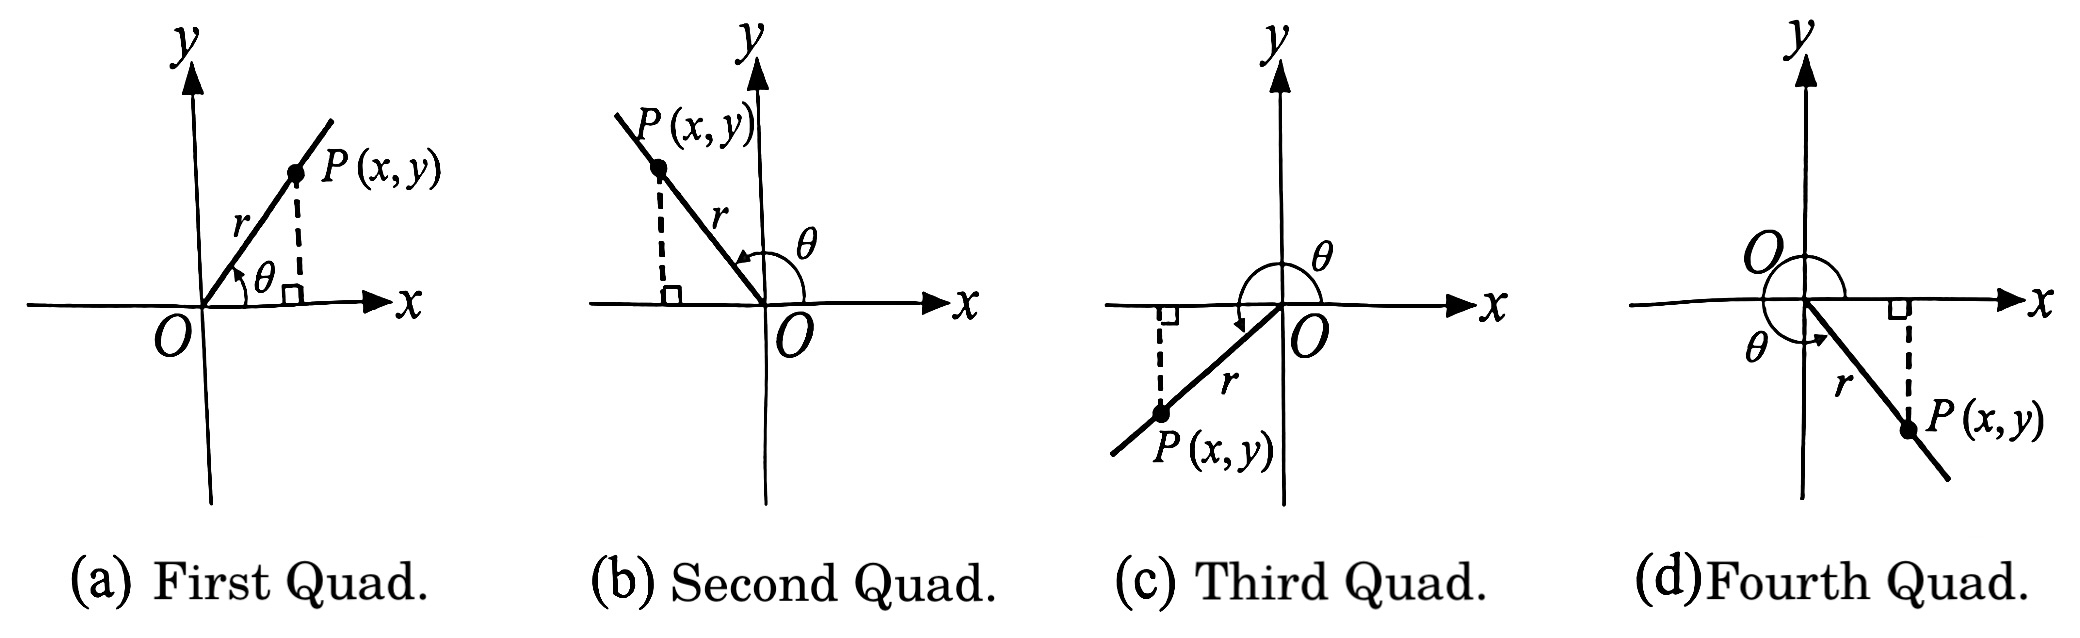
\includegraphics[width=0.8\textwidth]{assets/9-4.jpg}
\end{center}
\vspace{-1em}

As shown in the figure above, place an arbitrary angle $\theta$ in a coordinate system, and let the vertex of the angle as the origin, and the initial side of the angle lie on the positive x-axis. Take any point $P(x, y)$ on the terminal side of angle $\theta$ other than the origin, and let $r = OP = \sqrt{x^2 + y^2}$. Then, the trigonometric functions of angle $\theta$ are defined as follows:
\begin{info}[Trigonometric Functions of Arbitrary Angles]
    \begin{flalign*}
        \text{Sine} & \sin\theta = \dfrac{y}{r} & \text{Cosine} &\cos\theta = \dfrac{x}{r} &\\
        \text{Tangent} & \tan\theta = \dfrac{y}{x},\ x \neq 0 & \text{Cotangent} & \cot\theta = \dfrac{x}{y},\ y \neq 0 &\\
        \text{Secant} & \sec\theta = \dfrac{r}{x},\ x \neq 0 & \text{Cosecant} & \operatorname{cosec}\theta = \dfrac{r}{y},\ y \neq 0 &&&&&
    \end{flalign*}
\end{info}

\begin{question}
    Given that the terminal side of angle $\theta$ passes through point $P(2, -3)$, find the six trigonometric functions of angle $\theta$.

    \sol{}
    \vspace{-3em}
    \begin{multicols}{2}
        \begin{flalign*}
            \because\ &x=2, y=-3 &\\
            \therefore\ &r=\sqrt{2^2+(-3)^2} \\
            &\ \ =\sqrt{13} 
        \end{flalign*}
        \vspace{-3em}
        \begin{flalign*}
            \therefore\ \sin \theta&=\dfrac{y}{r}=\dfrac{-3}{\sqrt{13}}=-\dfrac{3 \sqrt{13}}{13} \\
            \cos \theta&=\dfrac{x}{r}=\dfrac{2}{\sqrt{13}}=\dfrac{2 \sqrt{13}}{13} \\
            \tan \theta&=\dfrac{y}{x}=\dfrac{-3}{2}=-\dfrac{3}{2} \\
            \cot \theta&=\dfrac{x}{y}=\dfrac{2}{-3}=-\dfrac{2}{3} \\
            \sec \theta&=\dfrac{r}{x}=\dfrac{\sqrt{13}}{2} \\
            \operatorname{cosec} \theta&=\dfrac{r}{y}=-\dfrac{\sqrt{13}}{3} &
        \end{flalign*}
        \vspace{1em}
            
        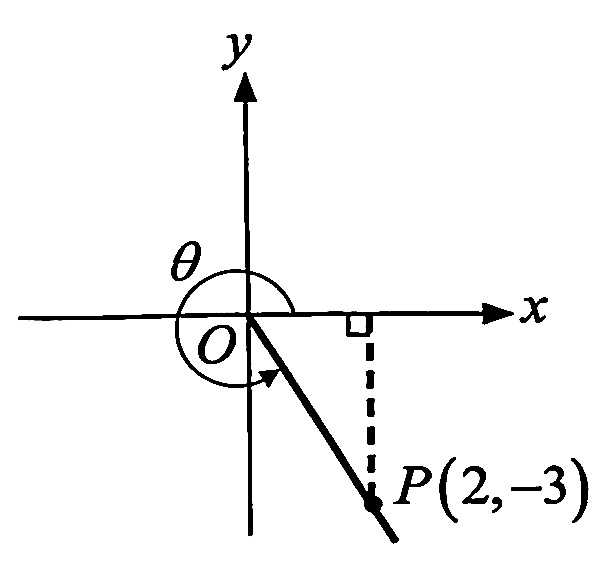
\includegraphics[width=0.24\textwidth]{assets/9-5.jpg}
    \end{multicols}
\end{question}
\begin{think}
    
    \noindent What is the relationship between the six trigonometric functions of an angle?
\end{think}

\practice{9.1b}

\vspace{-1em}
Given that $P\left(-\sqrt{3}, -1\right)$ is a point on the terminal side of angle $\alpha$, find the six trigonometric functions of angle $\alpha$.

\begin{explore}[Exploration Activity 1]
    
    \noindent \textbf{Definition of trigonometric functions in a unit circle}

    \noindent Given a circle with radius $r=1$ and center at the origin, take the intersection point $P(x, y)$ of the terminal side of angle $\theta$ with the circle. Since $r = OP = 1$, we have $\sin\theta = y$, $\cos\theta = x$, i.e. the vertical and horizontal coordinates of point $P$ are the sine and cosine of angle $\theta$ respectively.

    \noindent Now, open these GeoGebra Applet, inspect in action on how to define the sine function, cosine function, and tangent function using the coordinates of the point on the terminal side of $\theta$.

    \noindent \textbf{Tools:}
    \vspace{-1em}
    \begin{itemize}[leftmargin=*]
        \item Sine function and unit circle: \url{https://www.geogebra.org/m/xxjshdwq}
        \item Cosine function and unit circle: \url{https://www.geogebra.org/m/aajvmasj}
        \item Tangent function and unit circle: \url{https://www.geogebra.org/m/u6qg8x4z}
    \end{itemize}
\end{explore}

\vspace{-0.5em}
\subsection*{Trigonometric Values of Arbitrary Angles}

When defining the trigonometric functions of arbitrary angles, the initial side of the angle is fixed on the positive x-axis, and according to the size of $\theta$ and the direction of the rotation, the terminal side of the angle can be in any quadrant or on the coordinate axes. From this definition, we know that the value of the trigonometric functions of an angle is only determined by the location of the terminal side of the angle. Hence, $\theta$ and $\theta pm k \cdot 360^\circ$, $k \in \mathbb{Z}$ have the same value of trigonometric functions.

Regardless of the quadrant to which the terminal side of angle $\theta$ belongs, the value of $r$ is always positive ($r > 0$), while the value of $x$ and $y$ can be positive or negative, as shown in the table figure below. Hence, the trigonometric values of an angle can be positive or negative, depending on the quadrant to which the terminal side of the angle belongs, as shown in the table below.
\begin{vwcol}[widths={0.2,0.8}, sep=4mm, justify=flush, rule=0pt]
    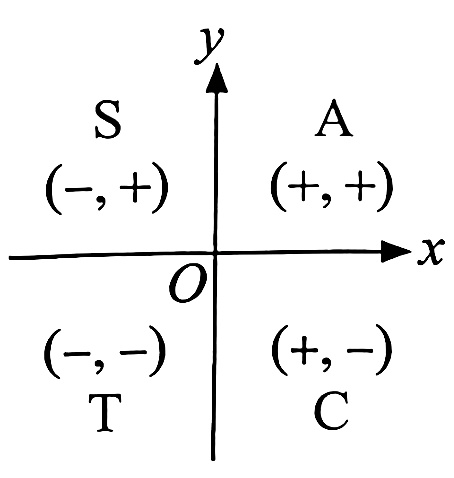
\includegraphics[width=0.2\linewidth]{assets/9-6.jpg}

    \parbox{0.8\textwidth}{\vspace{1.5em}\begin{tabular}{|c|c|c|c|c|}
        \hline  & First Quadrant & Second Quadrant & Third Quadrant & Fourth Quadrant \\
        \hline $\sin \theta$ & + & + & - & - \\
        \hline $\cos \theta$ & + & - & - & + \\
        \hline $\tan \theta$ & + & - & + & - \\
        \hline
        \end{tabular}}
\end{vwcol}
\begin{warn}[Note]
    
    \vspace{-1em} 
    \noindent $A$: All trigonometric values are positive

    \vspace{-1em}
    \noindent $S$: $\sin \theta$ is positive $\qquad$ $T$: $\tan \theta$ is positive $\qquad$ $C$: $\cos \theta$ is positive
    
    \vspace{-1em}
    \noindent The sign of the values of $\operatorname{cosec} \theta$, $\sec \theta$, and $\cot \theta$ are the same as the signs of $\sin \theta$, $\cos \theta$, and $\tan \theta$ respectively.
\end{warn}

\practice{9.1c}
\begin{enumerate}
    \item Without using a calculator, determine which quadrant the angle $\theta$ belongs to, and hence, find the sign of $\sin \theta$, $\cos \theta$, and $\tan \theta$:
    
    \begin{center}
        \begin{tabular}{|c|c|c|c|c|c|}
            \cline { 2 - 6 } \multicolumn{1}{c|}{} & $\theta$ & Quadrant & $\sin \theta$ & $\cos \theta$ & $\tan \theta$ \\
            \hline Example & $330^{\circ}$ & 4th & - & + & - \\
            \hline (a) & $-160^{\circ}$ & & & & \\
            \hline (b) & $210^{\circ}$ & & & & \\
            \hline (c) & $1068^{\circ}$ & & & & \\
            \hline (d) & $\dfrac{3 \pi}{4}$ & & & & \\
            \hline (e) & -5 & & & & \\
            \hline
            \end{tabular}
    \end{center}
    \item According to the following criteria, determine which quadrant the angle $\theta$ belongs to:
    \begin{multicols}{2}
        \begin{enumerate}[label=(\alph*)]
            \item $\cot \theta<0$
            \item $\sin \theta>0$ and $\cos \theta<0$
            \item $\sec \theta<0$ and $\tan \theta>0$
            \item $\sin \theta \cdot \cot \theta>0$
        \end{enumerate}
    \end{multicols}
\end{enumerate}
\begin{question}
    Given that $\sin\theta = \dfrac{4}{5}$. Without finding the value of angle $\theta$, find the value of $\tan\theta$ and $\sec\theta$.

    \sol{}

    \noindent Given that $\sin\theta > 0$, hence $\theta$ belongs to the first or second quadrant. 

    \vspace{-1em}
    \begin{multicols}{2}
        \noindent Let $r = 5$, $y = 4$
        \vspace{-1em}
    \begin{enumerate}[label=(\roman*),leftmargin=*]
        \item If $\theta$ is in the first quadrant, then $x = \sqrt{5^2 - 4^2} = 3$,
        
        $\therefore$ $\tan\theta = \dfrac{4}{3}$, $\sec\theta = \dfrac{5}{3}$

        \item If $\theta$ is in the second quadrant, then $x = -\sqrt{5^2 - 4^2} = -3$,
        
        $\therefore$ $\tan\theta = -\dfrac{4}{3}$, $\sec\theta = -\dfrac{5}{3}$
    \end{enumerate}
    \vfill\null

    \begin{center}
        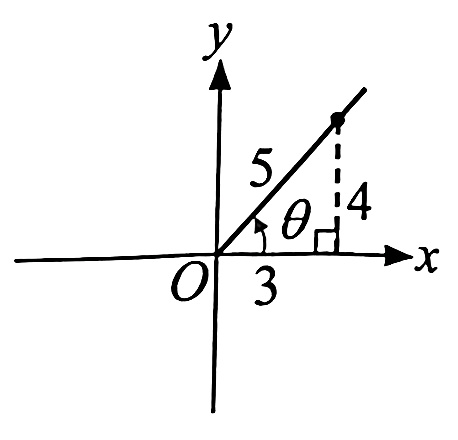
\includegraphics[width=0.2\textwidth]{assets/9-7.jpg}
    \end{center}
    \vspace{-3em}
    \begin{center}
        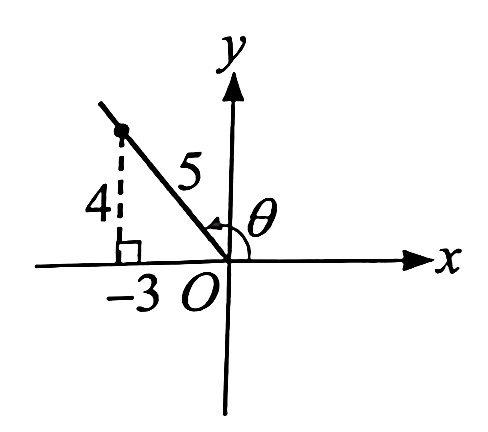
\includegraphics[width=0.21\textwidth]{assets/9-8.jpg}
    \end{center}
    \end{multicols}
\end{question}

\vspace{-1em}
In Example 3, we can see that there is an acute angle between the terminal side of $\theta$ and the $x$-axis.
\begin{center}
    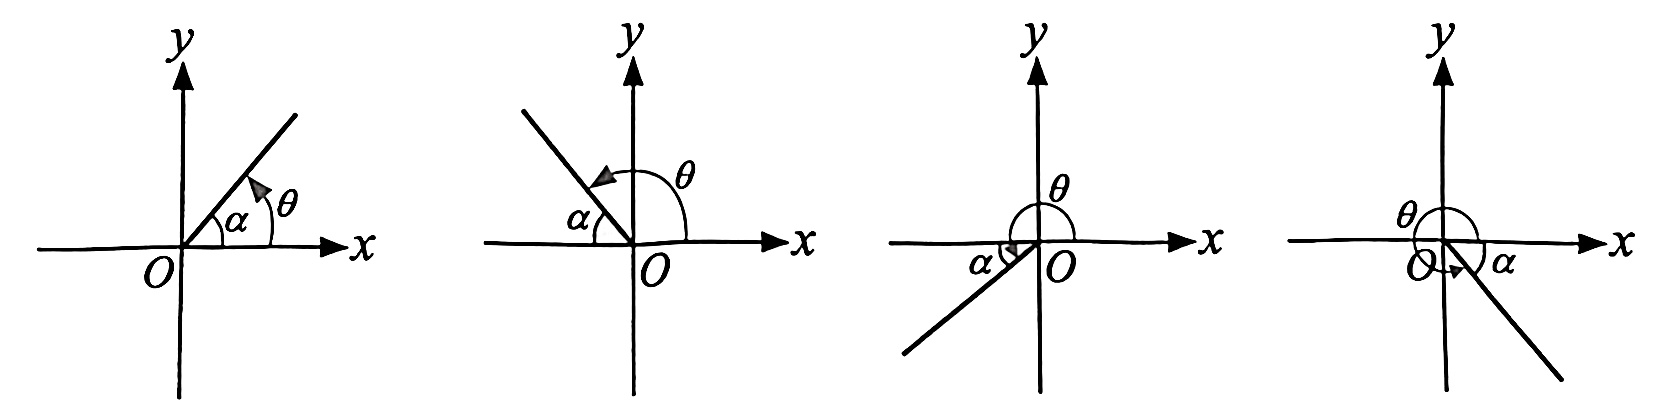
\includegraphics[width=0.8\textwidth]{assets/9-9.jpg}
\end{center}

As shown in the figure, no matter which quadrant $\theta$ belongs to, the acute angle $\alpha$ between its terminal side and the $x$-axis is known as the \textbf{associated acute angle} or \textbf{reference angle} of $\theta$. Since the acute angle $\alpha$ is in the first quadrant, the trigonometric values of $\alpha$ are always positive, and we can see that the absolute trigonometric values of $\theta$ is the same as the trigonometric values of $\alpha$. Hence, using the sign of the trigonometric functions and the trigonometric values of the reference angle, we can convert the problems of finding the trigonometric values of arbitrary angles to finding the trigonometric values of acute angles.

\begin{question}
    Convert the following expressions into trigonometric functions of acute angles:
    \vspace{-1em}
    \begin{multicols}{3}
        \begin{enumerate}[label=(\alph*)]
            \item $\sin 565^\circ$
            \item $\operatorname{cosec}\left(-285^\circ\right)$
            \item $\cos\dfrac{9\pi}{10}$
        \end{enumerate}
    \end{multicols}

    \sol{}
    \begin{enumerate}[label=(\alph*)]
        \item \begin{multicols}{2}
            $565^\circ$ is in the third quadrant, $\sin 565^\circ < 0$, the reference angle is $25^\circ$,

            $\therefore$ $\sin 565^\circ = -\sin 25^\circ$

            \vfill\null

            \begin{center}
                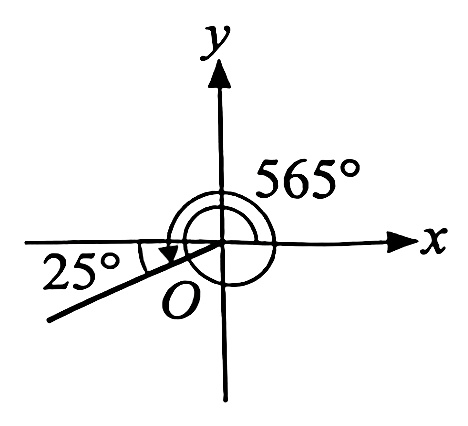
\includegraphics[width=0.2\textwidth]{assets/9-10.jpg}
            \end{center}
        \end{multicols}

        \item \begin{multicols}{2}
            $-285^\circ$ is in the first quadrant, $\operatorname{cosec}(-285^\circ) > 0$, the reference angle is $75^\circ$,

            $\therefore$ $\operatorname{cosec}(-285^\circ) = \operatorname{cosec}75^\circ$

            \vfill\null
            \begin{center}
                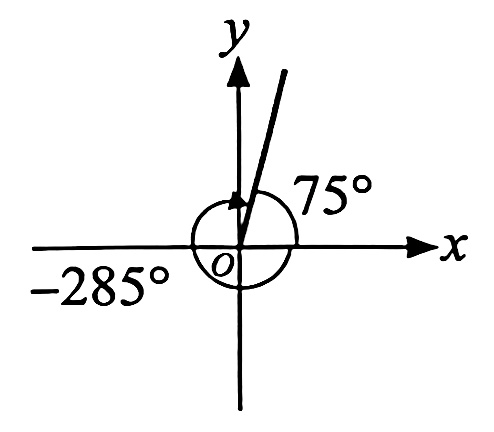
\includegraphics[width=0.2\textwidth]{assets/9-11.jpg}
            \end{center}
        \end{multicols}

        \item \begin{multicols}{2}
            $\dfrac{9\pi}{10}$ is in the second quadrant, $\cos\dfrac{9\pi}{10} < 0$, the reference angle is $\dfrac{\pi}{10}$,

            $\therefore$ $\cos\dfrac{9\pi}{10} = -\cos\dfrac{\pi}{10}$

            \vfill\null
            \begin{center}
                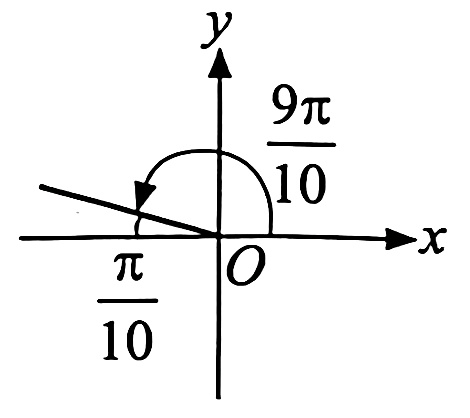
\includegraphics[width=0.2\textwidth]{assets/9-12.jpg}
            \end{center}
        \end{multicols}
    \end{enumerate}
\end{question}

\newpage
\begin{question}
    \begin{multicols}{4}
        \begin{enumerate}[label=(\alph*)]
            \item $\sin 300^\circ$
            \item $\tan\left(-150^\circ\right)$
            \item \vspace*{-1.1em}$\cot\left(\dfrac{17\pi}{4}\right)$
            \item $\cos^2 210^\circ$
        \end{enumerate}
    \end{multicols}

    \sol{}
        \begin{enumerate}[label=(\alph*),leftmargin=*]
            \item \begin{multicols}{2}
                $\begin{aligned}[t]
                    \sin 300^\circ &= -\sin 60^\circ \\
                    &= -\dfrac{\sqrt{3}}{2}
                \end{aligned}$
                \vfill\null
                \begin{center}
                    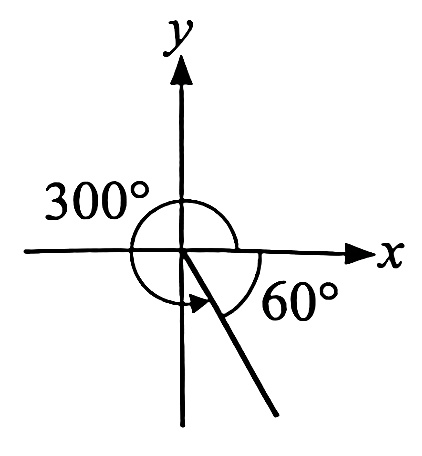
\includegraphics[width=0.2\textwidth]{assets/9-13.jpg}
                \end{center}
            \end{multicols}
            \vspace{-3em}
            \item \begin{multicols}{2}
                $\begin{aligned}[t]
                    \tan\left(-150^\circ\right) &= \tan 30^\circ \\
                    &= \dfrac{\sqrt{3}}{3}
                \end{aligned}$
                \vfill\null
                \begin{center}
                    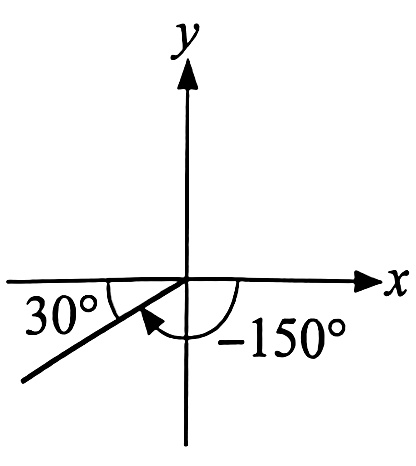
\includegraphics[width=0.2\textwidth]{assets/9-14.jpg}
                \end{center}
            \end{multicols}
            \vspace{-3em}
            \item \begin{multicols}{2}
                $\begin{aligned}[t]
                    \cot\left(\dfrac{17\pi}{4}\right) &= \cot\dfrac{\pi}{4} \\
                    &= 1
                \end{aligned}$
                \vfill\null
                \begin{center}
                    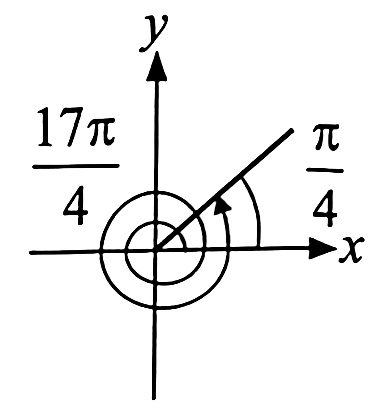
\includegraphics[width=0.2\textwidth]{assets/9-15.jpg}
                \end{center}
            \end{multicols}
            \vspace{-3em}
            \item \begin{multicols}{2}
                $\begin{aligned}[t]
                    \cos^2 210^\circ &= \cos^2 30^\circ \\
                    &= \dfrac{3}{4}
                \end{aligned}$
                \vfill\null
                \begin{center}
                    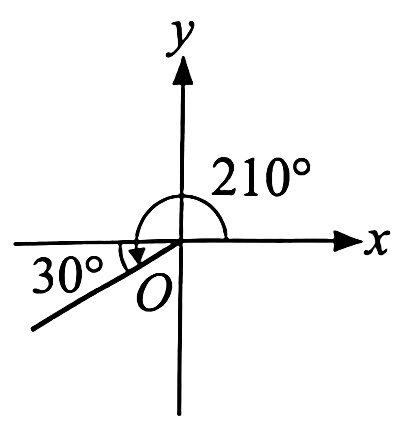
\includegraphics[width=0.2\textwidth]{assets/9-16.jpg}
                \end{center}
            \end{multicols}
        \end{enumerate}
\end{question}

\begin{question}
    \begin{multicols}{2}
        Given that $\cos\theta = \cos 50^\circ$, find the value of $\theta$.

    \sol{}

    \noindent $\because$ $\cos 50^\circ > 0$, $\therefore$ $\theta$ is in the first or fourth quadrant.
    
    \vspace{-1em}
    \noindent $\because$ Reference angle is $50^\circ$,

    \vspace{-1em}
    \noindent $\therefore$ $\theta = 50^\circ$ or $\theta = 360^\circ - 50^\circ = 310^\circ$

    \begin{center}
        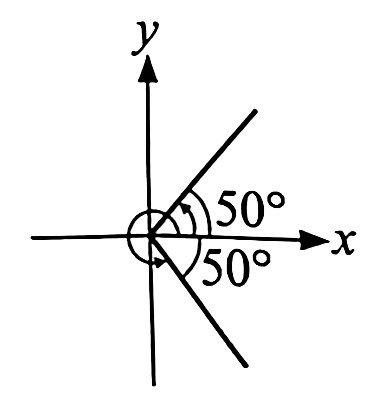
\includegraphics[width=0.2\textwidth]{assets/9-17.jpg}
    \end{center}
    \end{multicols}
\end{question}

\practice{9.1d}
\begin{enumerate}
    \item Let $180^\circ < A < 270^\circ$ and $\cot A = \dfrac{24}{7}$. Without finding the angle $A$, find the values of $\cos A$ and $\operatorname{cosec} A$.

    \item Without using a calculator, find the values of the following trigonometric functions:
    \begin{multicols}{4}
        \begin{enumerate}[label=(\alph*)]
            \item $\cos 150^\circ$
            \item $\sec (-330^\circ)$
            \item $\sin 690^\circ$
            \item \vspace*{-1.8em} $\cot \left(-\dfrac{5 \pi}{4}\right)$
            \end{enumerate}
    \end{multicols}
    \vspace{-1.5em}
    \item Given $\sin \alpha = -\sin \dfrac{\pi}{8}$, and $0 \leq \alpha \leq 2 \pi$, find the value of $\alpha$.

\item \begin{enumerate}[label=(\alph*)]
\item Given $\sin 16^\circ \approx 0.2756$, find $\sin 164^\circ$.
\item Given $\cos 696^\circ \approx 0.9135$, find $\cos 24^\circ$.
\end{enumerate}
\end{enumerate}

\begin{vwcol}[widths={0.6,0.4}, sep=4mm, justify=flush, rule=0pt]
    We have previously discussed the signs of the trigonometric functions in different quadrants. In the next section, we will discuss the situations where the terminal side of the angle lies on the coordinate axes. Reviewing exploration activity 1, we can see that (as shown in the figure to the right):
    
    \noindent \parbox{0.58\textwidth}{\begin{enumerate}[label=(\roman*),leftmargin=*]
        \item When the terminal side of the angle lies on the $x$-axis, the $y$-coordinate of the intersection point $P$ is 0, hence, $\cot\theta$ and $\operatorname{cosec}\theta$ are undefined.
        \item When the terminal side of the angle lies on the $y$-axis, the $x$-coordinate of the intersection point $P$ is 0, hence, $\tan\theta$ and $\sec\theta$ are undefined.
    \end{enumerate}}
    
    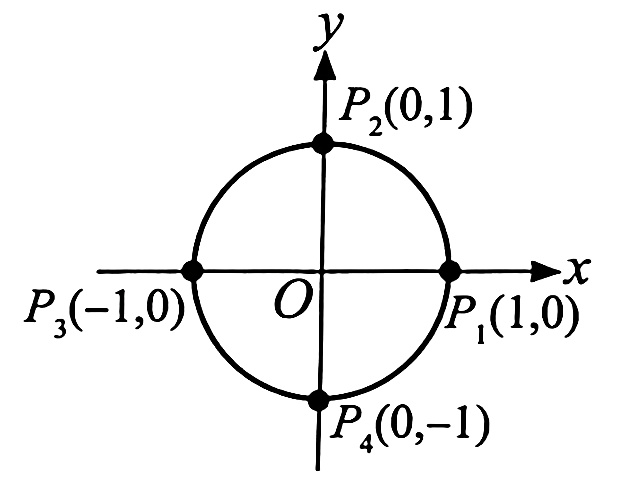
\includegraphics[width=0.34\linewidth]{assets/9-18.jpg}
\end{vwcol}
\vspace{-2em}
Listed in the following table are the sine, cosine, and tangent values of $0^\circ$, $90^\circ$, $180^\circ$, and $270^\circ$:
\begin{center}
    \begin{tabular}{|c|c|c|c|c|}
        \hline$\theta$ & $0^{\circ}$ & $90^{\circ}$ & $180^{\circ}$ & $270^{\circ}$ \\
        \hline $\sin \theta$ & 0 & 1 & 0 & -1 \\
        \hline $\cos \theta$ & 1 & 0 & -1 & 0 \\
         \hline $\tan \theta$ & 0 & undefined & 0 & undefined \\
        \hline
        \end{tabular}
\end{center}

\practice{9.1e}

Complete the following table:
\begin{center}
    \begin{tabularx}{0.8\textwidth}{|Y|Y|Y|Y|Y|}
        \hline$\theta$ & $0$ & $\dfrac{\pi}{2}$ & $\pi$ & $\dfrac{3 \pi}{2}$ \\
        \hline $\cot \theta$ & & & & \\
        \hline $\sec \theta$ & & & & \\
        \hline $\operatorname{cosec} \theta$ & & & & \\
        \hline
        \end{tabularx}
\end{center}

\newpage

\exercise{9.1}

\begin{enumerate}
    \item Determine in which quadrant the terminal side of each of the following angles lies:
    \begin{multicols}{4}
        \begin{enumerate}[label=(\alph*)]
            \item $840^\circ$
            \item $-190^\circ$
            \item \vspace*{-1.2em}$\dfrac{7 \pi}{4}$
            \item $-2$
            \end{enumerate}
    \end{multicols}

    \item Given that the terminal side of angle $\alpha$ passes through the following points, find the six trigonometric function values of $\alpha$:
    \begin{multicols}{2}
        \begin{enumerate}[label=(\alph*)]
            \item $(-8,-6)$
            \item $(-2,1)$
            \end{enumerate}
    \end{multicols}

    \item Without using a calculator, determine whether the following trigonometric values are positive or negative:
    \begin{multicols}{4}
        \begin{enumerate}[label=(\alph*)]
            \item $\cos 250^\circ$
            \item $\operatorname{cosec} \left(-1300^\circ\right)$
            \item $\tan 4$
            \item $\sin \left(-\dfrac{13}{3} \pi\right)$
            \end{enumerate}
    \end{multicols}

    \item Determine the quadrant to which angle $\theta$ belongs based on the following conditions:
    \begin{multicols}{2}
        \begin{enumerate}[label=(\alph*)]
            \item \vspace*{-2.4em}$\cos \theta = \dfrac{1}{3}$
            \item $\cos \theta$ and $\operatorname{cosec} \theta$ have the same sign
            \end{enumerate}  
    \end{multicols}
    \begin{multicols}{2}
        \begin{enumerate}[label=(\alph*),start=3]
            \item $\dfrac{\sin \theta}{\cot \theta} < 0$
            \item \vspace*{-0.3em}$\tan^2 \theta = 3$
        \end{enumerate}
    \end{multicols}

    \item If $\sec \alpha = -\dfrac{17}{15}$, without finding the angle $\alpha$, find the values of $\sin \alpha$ and $\tan \alpha$.

    \item If $\sin \theta = k$, where $k < 0$ and $\cos \theta > 0$, express $\tan \theta$ in terms of $k$.
    
    \item Express the following trigonometric functions as acute angle trigonometric functions:
    \begin{multicols}{4}
        \begin{enumerate}[label=(\alph*)]
            \item $\operatorname{cosec} 186^\circ$
            \item $\cot \left(-505^\circ\right)$
            \item $\sin 7.6 \pi$
            \item $\cos \left(-\dfrac{59}{17} \pi\right)$
            \end{enumerate}
    \end{multicols}

    \item Given $0 \leq \theta \leq 360^\circ$, without using a calculator, find the value of $\theta$ in each of the following equations:
    \begin{multicols}{2}
        \begin{enumerate}[label=(\alph*)]
            \item $\sin \theta = \sin 68^\circ$
            \item $\sec \theta = -\sec 34^\circ$
            \end{enumerate}
    \end{multicols}
\end{enumerate}
\begin{enumerate}[start=7]
    \begin{vwcol}[widths={0.8,0.2}, sep=4mm, justify=flush, rule=0pt]
        \parbox{0.7\textwidth}{\item As shown in the diagram on the right, in a right triangle $\triangle ABC$ where $BC = 2$ and $DC = t$, find the values of $\sin \angle BDA$ and $\cot \angle BDA$.

        \vspace{1em}
        \item Without using a calculator, evaluate the following expressions:
        
        \noindent\parbox{0.8\textwidth}{\begin{enumerate}[label=(\alph*)]
            \item $\sin 135^\circ + \cos 225^\circ + \sec 180^\circ + \operatorname{cosec} 90^\circ$
            \item $\sin 120^\circ + \cos^2 420^\circ + \tan 225^\circ - \operatorname{cosec}^2 240^\circ$
            \item $\sin \dfrac{25 \pi}{6} + \cos \dfrac{25 \pi}{6} + \tan \left(-\dfrac{25}{4} \pi\right) - \cos 2 \pi$
            \end{enumerate}}}
    
        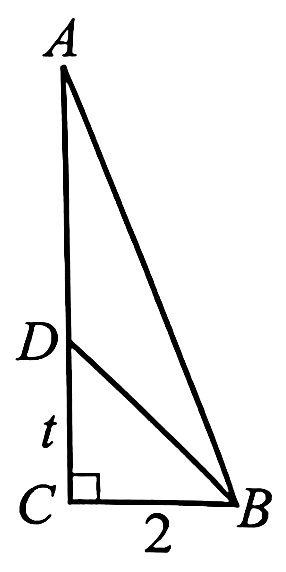
\includegraphics[width=0.14\textwidth]{assets/9-19.jpg}
    \end{vwcol}
\end{enumerate}

\newpage

\section{Induction Formulas of Trigonometric Functions}

In the last section, we discovered that the trigonometric functions of an arbitrary angle are cyclic, and each respective trigonometric value of the angle with the same terminal side is the same. This can be expressed in the following formulas, where $\theta$ is an arbitrary angle, $k \in \mathbb{Z}$, and assuming that the trigonometric functions are defined:

\begin{info}[Trigonometric Values of $\theta + k \cdot 360^\circ$ and $\theta$]
    \begin{align*}
        \sin(\theta + k \cdot 360^\circ) = \sin \theta \qquad \cos(\theta + k \cdot 360^\circ) = \cos \theta \qquad \tan(\theta + k \cdot 360^\circ) = \tan \theta 
    \end{align*}
    \noindent When $k = 1$, we have
    \begin{align*}
        \sin(360^\circ + \theta) = \sin \theta \qquad \cos(360^\circ + \theta) = \cos \theta \qquad \tan(360^\circ + \theta) = \tan \theta
    \end{align*}
\end{info}
With the relationship above, we can convert each trigonometric function to the trigonometric functions of an angle from $0^\circ$ to $360^\circ$ (or $0$ to $2\pi$), then use the reference angle to convert the them to the trigonometric functions of an acute angle to calculate the trigonometric values.

However, apart from using complementary angles, do we have any other ways to convert trigonometric functions of arbitrary angle into trigonometric functions of acute angles for calculation? Actually, we can express an angle whose terminal side lies on the coordinate axes in the form of $k \cdot 90^{\circ}$, so any arbitrary angle can be written as $k \cdot 90^{\circ} \pm \theta$, where $k \in \mathbb{Z}$. If we can find the relationship between the trigonometric values of an arbitrary angle $\theta$ and $k \cdot 90^{\circ} \pm \theta$, we can proceed with the conversion. Next, we are going to explore the relationships between the trigonometric values of $-\theta$, $90^{\circ} \pm \theta$, $180^{\circ} \pm \theta$, $270^{\circ} \pm \theta$, and the trigonometric values of $\theta$.

\begin{explore}[Exploration Activity 2]

\noindent\textbf{Purpose: } To explore trigonometric induction formulas.
\vspace{-1em}
\begin{enumerate}[label=(\alph*)]
    \item Trigonometric Relationship between $-\theta$ and $\theta$
    
    Angles $\theta$ and $-\theta$ represent rotations of the same magnitude but in opposite directions, hence their terminal sides are symmetric about the $x$-axis. Based on the definitions of trigonometric functions for any angle or other methods, find the trigonometric relationship between $-\theta$ and $\theta$.
    \item Trigonometric Relationship between $90^{\circ}+\theta$ and $\theta$
    
    Angle $90^{\circ}+\theta$ differs from angle $\theta$ by $90^{\circ}$. Based on the definition of trigonometric functions or other methods, find the trigonometric relationship between $90^{\circ}+\theta$ and $\theta$.

    \item Trigonometric Relationships between $90^{\circ}-\theta$, $180^{\circ} \pm \theta$, $270^{\circ} \pm \theta$, and $\theta$
    
    Since $90^{\circ}-\theta=90^{\circ}+(-\theta)$, utilize formulas derived from (a) and (b) to find the trigonometric relationship between $90^{\circ}-\theta$ and $\theta$.
    
    Similarly, treat $180^{\circ} \pm \theta$ as $90^{\circ}+\left(90^{\circ} \pm \theta\right)$ and $270^{\circ} \pm \theta$ as $90^{\circ}+\left(180^{\circ} \pm \theta\right)$, we can respectively obtain trigonometric relationships between $180^{\circ} \pm \theta$, $270^{\circ} \pm \theta$, and $\theta$.
\end{enumerate}
\vspace{-1em}
\textbf{Tool: }\url{https://www.geogebra.org/m/w7gx3umv}

\end{explore}

\newpage

From Exploratory Activity 2, we can derive the following formulas. These formulas hold true for any arbitrary θ that makes the trigonometric functions defined.

\begin{center}
    \parbox{0.36\textwidth}{\begin{info}[Trigonometric Values of $-\theta$ and $\theta$]
        \begin{align*}
            \sin(-\theta) &= -\sin \theta\\
            \cos(-\theta) &= \cos \theta\\
            \tan(-\theta) &= -\tan \theta
        \end{align*}
    \end{info}}
\end{center}

\begin{multicols}{2}
    \parbox{0.41\textwidth}{\begin{info}[Trigonometric Values of $90^{\circ} + \theta$ and $\theta$]
        \begin{align*}
            \sin(90^{\circ} + \theta) &= \cos \theta\\
            \cos(90^{\circ} + \theta) &= -\sin \theta\\
            \tan(90^{\circ} + \theta) &= -\cot \theta
        \end{align*}
    \end{info}}
    \parbox{0.41\textwidth}{\begin{info}[Trigonometric Values of $90^{\circ} - \theta$ and $\theta$]
        \begin{align*}
            \sin(90^{\circ} - \theta) &= \cos \theta\\
            \cos(90^{\circ} - \theta) &= \sin \theta\\
            \tan(90^{\circ} - \theta) &= \cot \theta
        \end{align*}
    \end{info}}
\end{multicols}

\begin{multicols}{2}
    \parbox{0.41\textwidth}{\begin{info}[Trigonometric Values of $180^{\circ} + \theta$ and $\theta$]
        \begin{align*}
            \sin(180^{\circ} + \theta) &= -\sin \theta\\
            \cos(180^{\circ} + \theta) &= -\cos \theta\\
            \tan(180^{\circ} + \theta) &= \tan \theta
        \end{align*}
    \end{info}}
    \parbox{0.41\textwidth}{\begin{info}[Trigonometric Values of $180^{\circ} - \theta$ and $\theta$]
        \begin{align*}
            \sin(180^{\circ} - \theta) &= \sin \theta\\
            \cos(180^{\circ} - \theta) &= -\cos \theta\\
            \tan(180^{\circ} - \theta) &= -\tan \theta
        \end{align*}
    \end{info}}
\end{multicols}

\begin{multicols}{2}
    \parbox{0.41\textwidth}{\begin{info}[Trigonometric Values of $270^{\circ} + \theta$ and $\theta$]
        \begin{align*}
            \sin(270^{\circ} + \theta) &= -\cos \theta\\
            \cos(270^{\circ} + \theta) &= \sin \theta\\
            \tan(270^{\circ} + \theta) &= -\cot \theta
        \end{align*}
    \end{info}}
    \parbox{0.41\textwidth}{\begin{info}[Trigonometric Values of $270^{\circ} - \theta$ and $\theta$]
        \begin{align*}
            \sin(270^{\circ} - \theta) &= -\cos \theta\\
            \cos(270^{\circ} - \theta) &= -\sin \theta\\
            \tan(270^{\circ} - \theta) &= \cot \theta
        \end{align*}
    \end{info}}
\end{multicols}

All the formulas in this section are known as the \textbf{induction formulas} of trigonometric functions. This induction formulas can be summarised as follows:

\noindent For the trigonometric values of $k \cdot 90^\circ \pm \theta$ ($k \in \mathbb{Z}$),
\vspace{-1em}
\begin{enumerate}[label=(\roman*)]
    \item When $k$ is even, its value is equal to the value of the function of the same name of theta, adding the sign of the original trigonometric value when treating $\theta$ as an acute angle.
    \item When $k$ odd, its value is equal to the value of the cofunction of theta, adding the sign of the original trigonometric value when treating $\theta$ as an acute angle. ($\sin\alpha$ and $\cos\alpha$, $\tan\alpha$ and $\cot\alpha$, $\sec\alpha$ and $\operatorname{cosec}\alpha$ are cofunctions of each other.)
\end{enumerate}

In the formulas above, changing the sine function to the cosecant function, the cosine function to the secant function, the formulas still hold true. 

\end{document}